\documentclass[11pt, a4paper]{article}
\usepackage{pdfpages}
\usepackage{parallel}
\usepackage[T2A]{fontenc}
\usepackage{ucs}
\usepackage[utf8x]{inputenc}
\usepackage[polish,english,russian]{babel}
\usepackage{hyperref}
\usepackage{rotating}
\usepackage[inner=2cm,top=1.8cm,outer=2cm,bottom=2.3cm,nohead]{geometry}
\usepackage{listings}
\usepackage{graphicx}
\usepackage{wrapfig}
\usepackage{longtable}
\usepackage{indentfirst}
\usepackage{array}
\usepackage{tikzsymbols}
\usepackage{soul}
\usepackage[ruled,vlined]{algorithm2e}
%\counterwithout{figure}{section} 

\usepackage{url}
\makeatletter
\g@addto@macro{\UrlBreaks}{\UrlOrds}
\makeatother

\newcolumntype{P}[1]{>{\raggedright\arraybackslash}p{#1}}
\frenchspacing
\usepackage{fixltx2e} %text sub- and superscripts
\usepackage{icomma} % коскі ў матэматычным рэжыме
\PreloadUnicodePage{4}

\newcommand{\longpage}{\enlargethispage{\baselineskip}}
\newcommand{\shortpage}{\enlargethispage{-\baselineskip}}

\def\switchlang#1{\expandafter\csname switchlang#1\endcsname}
\def\switchlangbe{
\let\saverefname=\refname%
\def\refname{Літаратура}%
\def\figurename{Іл.}%
}
\def\switchlangen{
\let\saverefname=\refname%
\def\refname{References}%
\def\figurename{Fig.}%
}
\def\switchlangru{
\let\saverefname=\refname%
\let\savefigurename=\figurename%
\def\refname{Литература}%
\def\figurename{Рис.}%
}

\hyphenation{admi-ni-stra-tive}
\hyphenation{ex-pe-ri-ence}
\hyphenation{fle-xi-bi-li-ty}
\hyphenation{Py-thon}
\hyphenation{ma-the-ma-ti-cal}
\hyphenation{re-ported}
\hyphenation{imp-le-menta-tions}
\hyphenation{pro-vides}
\hyphenation{en-gi-neering}
\hyphenation{com-pa-ti-bi-li-ty}
\hyphenation{im-pos-sible}
\hyphenation{desk-top}
\hyphenation{elec-tro-nic}
\hyphenation{com-pa-ny}
\hyphenation{de-ve-lop-ment}
\hyphenation{de-ve-loping}
\hyphenation{de-ve-lop}
\hyphenation{da-ta-ba-se}
\hyphenation{plat-forms}
\hyphenation{or-ga-ni-za-tion}
\hyphenation{pro-gramming}
\hyphenation{in-stru-ments}
\hyphenation{Li-nux}
\hyphenation{sour-ce}
\hyphenation{en-vi-ron-ment}
\hyphenation{Te-le-pathy}
\hyphenation{Li-nux-ov-ka}
\hyphenation{Open-BSD}
\hyphenation{Free-BSD}
\hyphenation{men-ti-on-ed}
\hyphenation{app-li-ca-tion}

\def\progref!#1!{\texttt{#1}}
\renewcommand{\arraystretch}{2} %Іначай формулы ў матрыцы зліпаюцца з лініямі
\usepackage{array}

\def\interview #1 (#2), #3, #4, #5\par{

\section[#1, #3, #4]{#1 -- #3, #4}
\def\qname{LVEE}
\def\aname{#1}
\def\q ##1\par{{\noindent \bf \qname: ##1 }\par}
\def\a{{\noindent \bf \aname: } \def\qname{L}\def\aname{#2}}
}

\def\interview* #1 (#2), #3, #4, #5\par{

\section*{#1\\{\small\rm #3, #4. #5}}
\ifx\ParallelWhichBox\undefined%
    \addcontentsline{toc}{section}{#1, #3, #4}%
\else%
\ifnum\ParallelWhichBox=0%
    \addcontentsline{toc}{section}{#1, #3, #4}%
\fi\fi%

\def\qname{LVEE}
\def\aname{#1}
\def\q ##1\par{{\noindent \bf \qname: ##1 }\par}
\def\a{{\noindent \bf \aname: } \def\qname{L}\def\aname{#2}}
}

\newcommand{\interviewfooter}[1]{
\vskip 1em
\noindent \textit{#1}
}

\switchlang{en}
\begin{document}

\title{1999 "--- Trackerball ProTrack 60i trackball}
\date{}
\maketitle
\selectlanguage{english}
The ProTrack 60i is manufactured by Trackerball, a former division of Marconi (the developer of the very first radar trackball in the 1940s to control the on-screen cursor of military radars), which became independent in 1995 \cite{history}.

\begin{figure}[h]
    \centering
    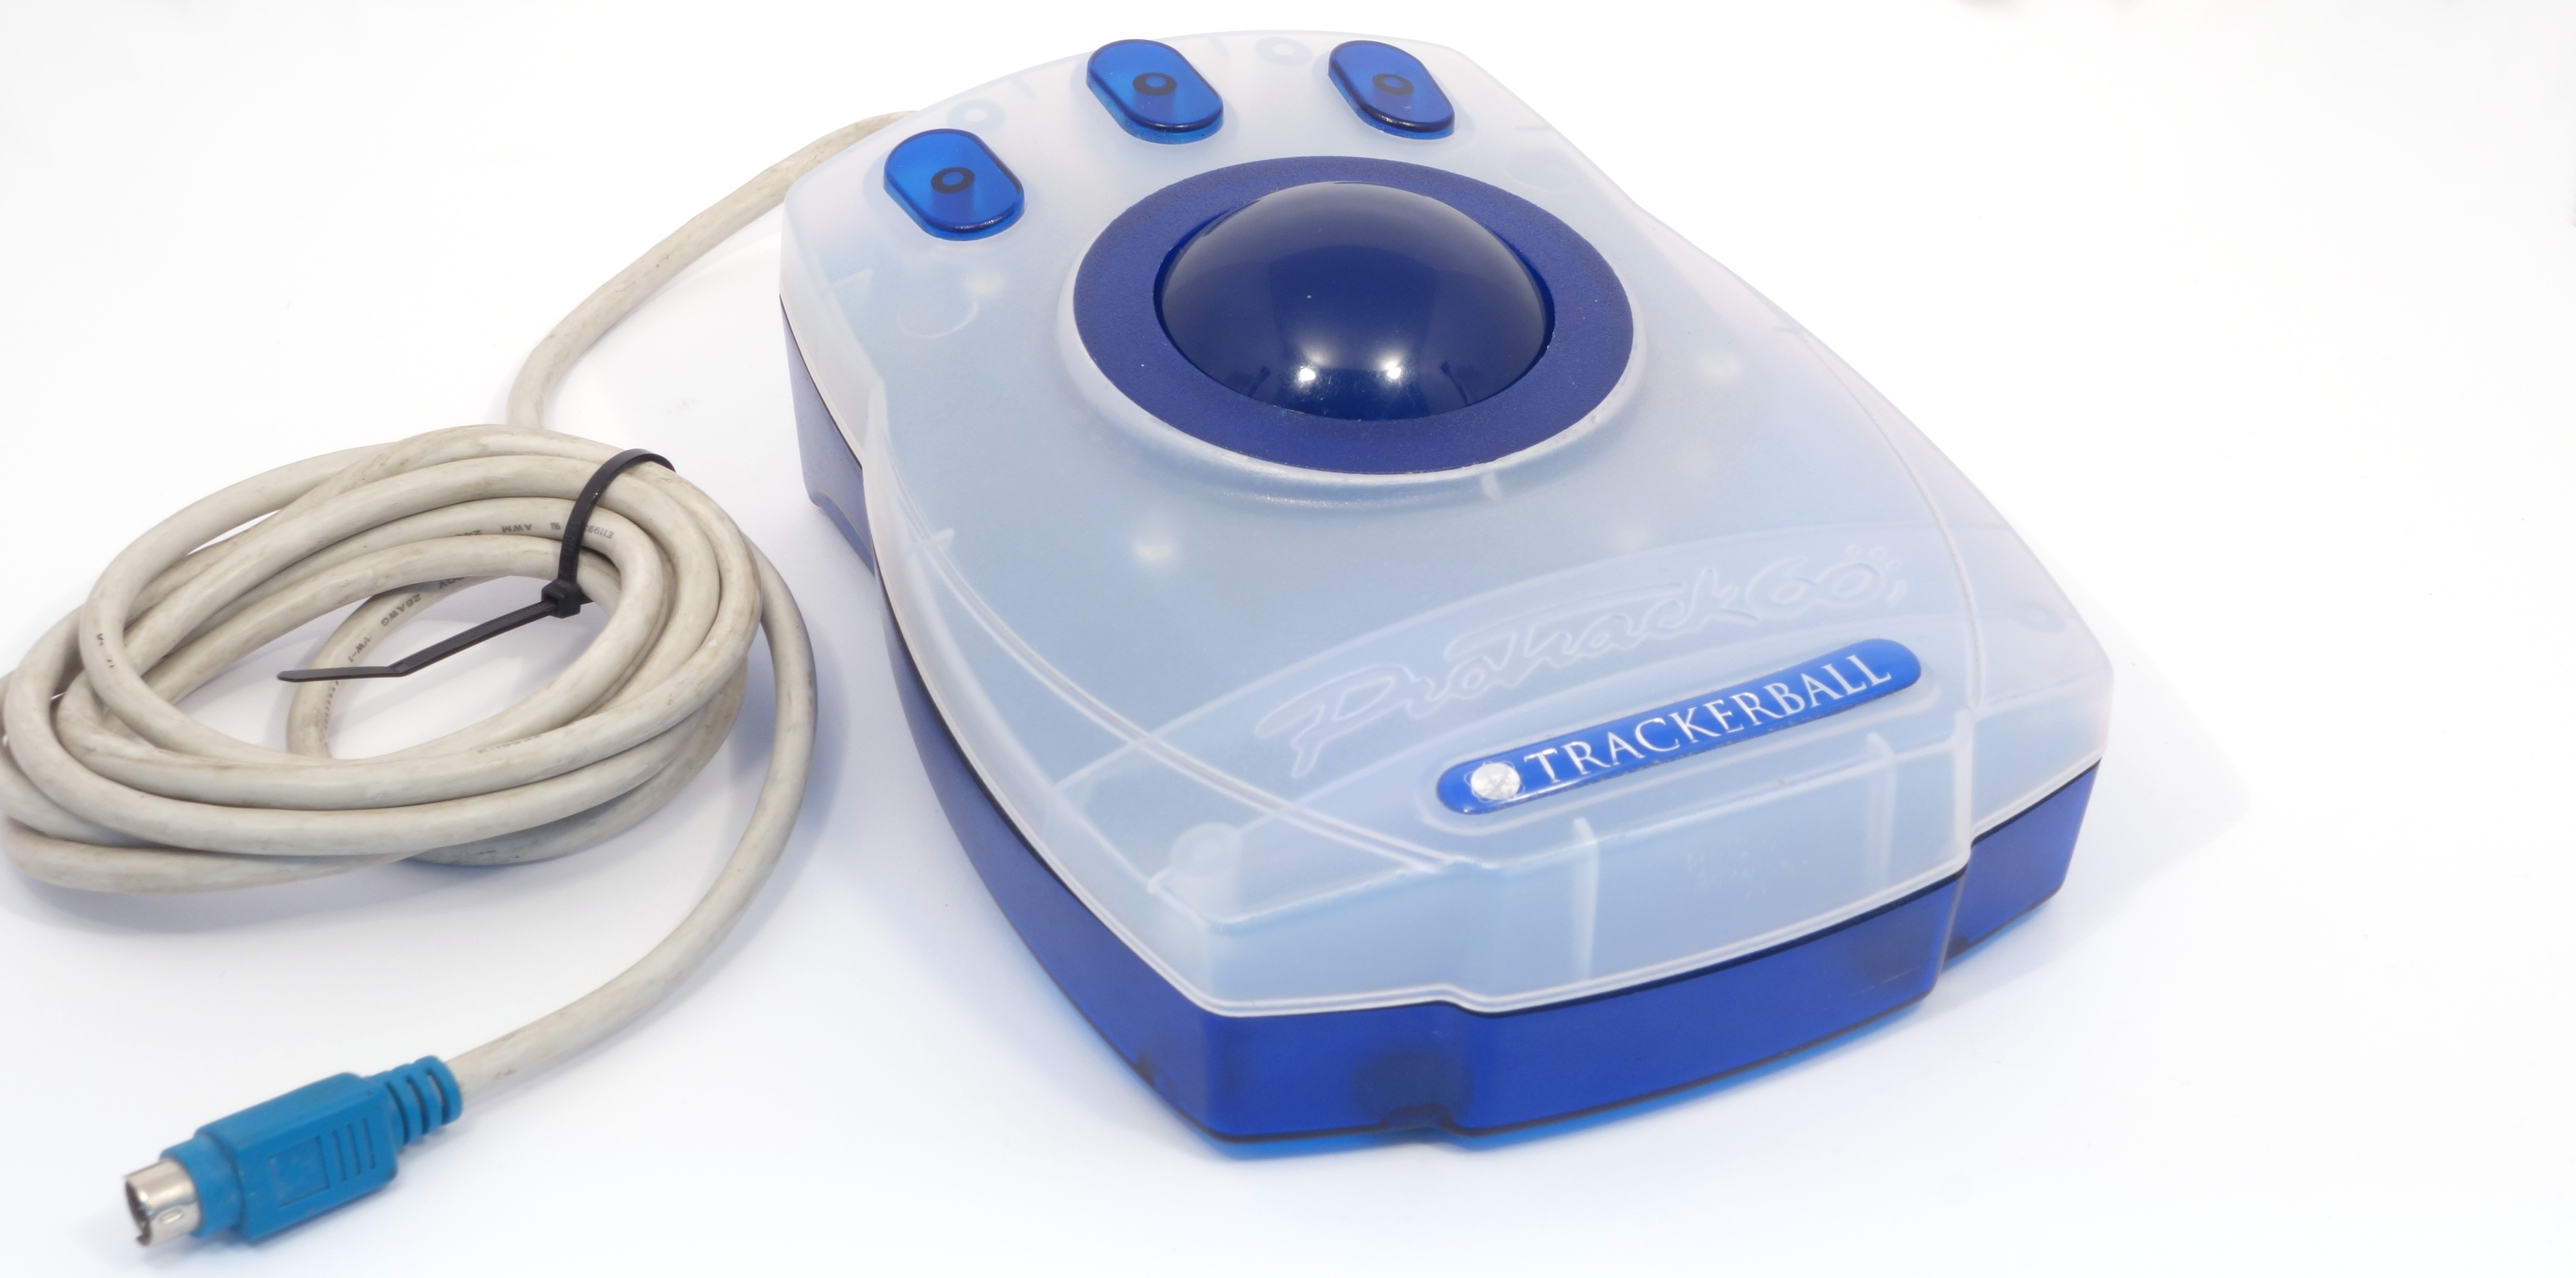
\includegraphics[scale=0.35]{1999_protrack_60i/monstr1_30.jpg}
    \caption{Trackerball ProTrack 60i trackball}
    \label{fig:ProTrack60i}
\end{figure}

The trackball was produced in two versions: the R60 (ProTrack 60) with a characteristic white body with a black ball and buttons, and the R60i (ProTrack 60i) with a translucent body and a blue backlit ball designed for use in dimly lit rooms, as shown in figure \ref {fig:ProTrack60i}. The most common connection interfaces are PS/2 and USB, however, the website of Cursor Controls, which Trackerball became a part of in 2000, also mentions RS-232, SUN and DEC interfaces \cite{trackerball,cursorcontrols}.

Note that this device is an extremely large trackball (figure \ref{fig:ProTrack60iSize}). The ball diameter is 63.5 mm (2.5 inches).

\begin{figure}[h]
    \centering
    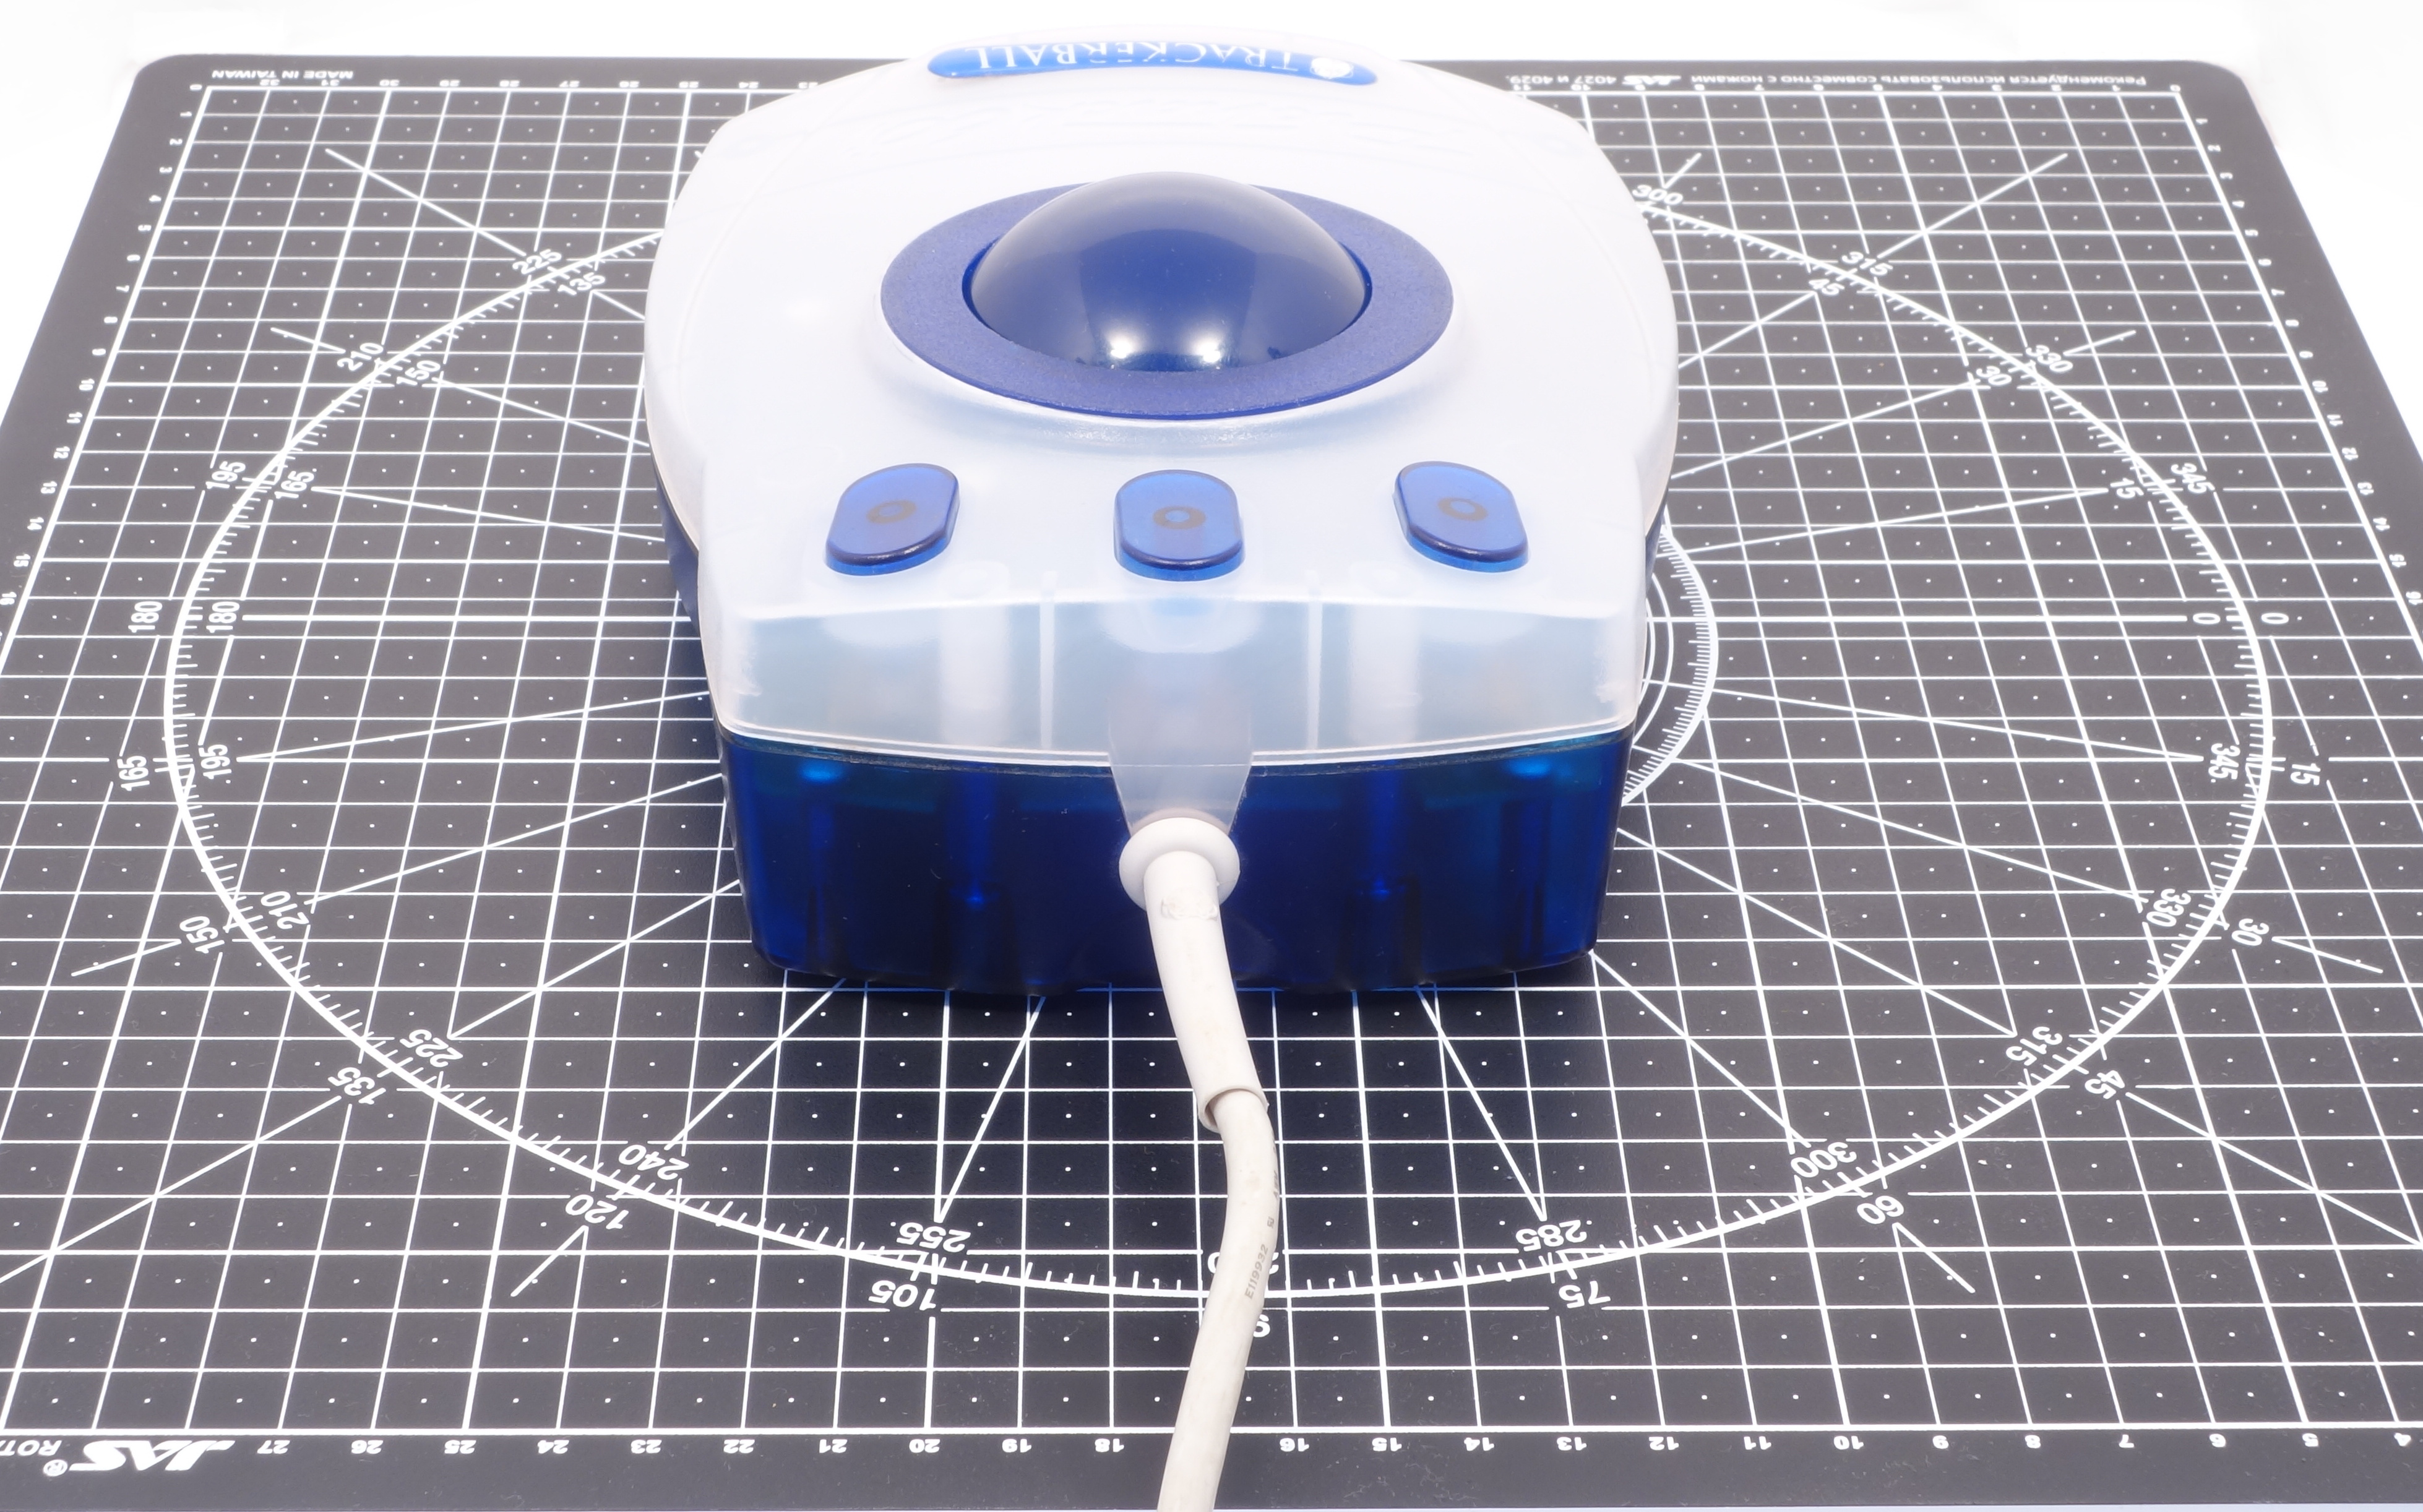
\includegraphics[scale=0.35]{1999_protrack_60i/monstr2.jpg}
    \caption{ProTrack 60i on a graduated pad with a grid step of 1~cm}
    \label{fig:ProTrack60iSize}
\end{figure}

The trackball is equipped with three buttons located on the opposite side from the user, behind the ball.
According to \cite{trackballfan}, this layout of the buttons minimizes the chance of accidentally pressing them when moving the ball, which is obviously important in industrial or military use of the trackball, but makes it difficult to drag-and-drop objects (which is not typical for such application areas).
The trackball does not have a scroll wheel, but the manufacturer's documentation mentions the ability to scroll with a ball, which is activated and deactivated by pressing the middle button.

\begin{figure}[h]
    \centering
    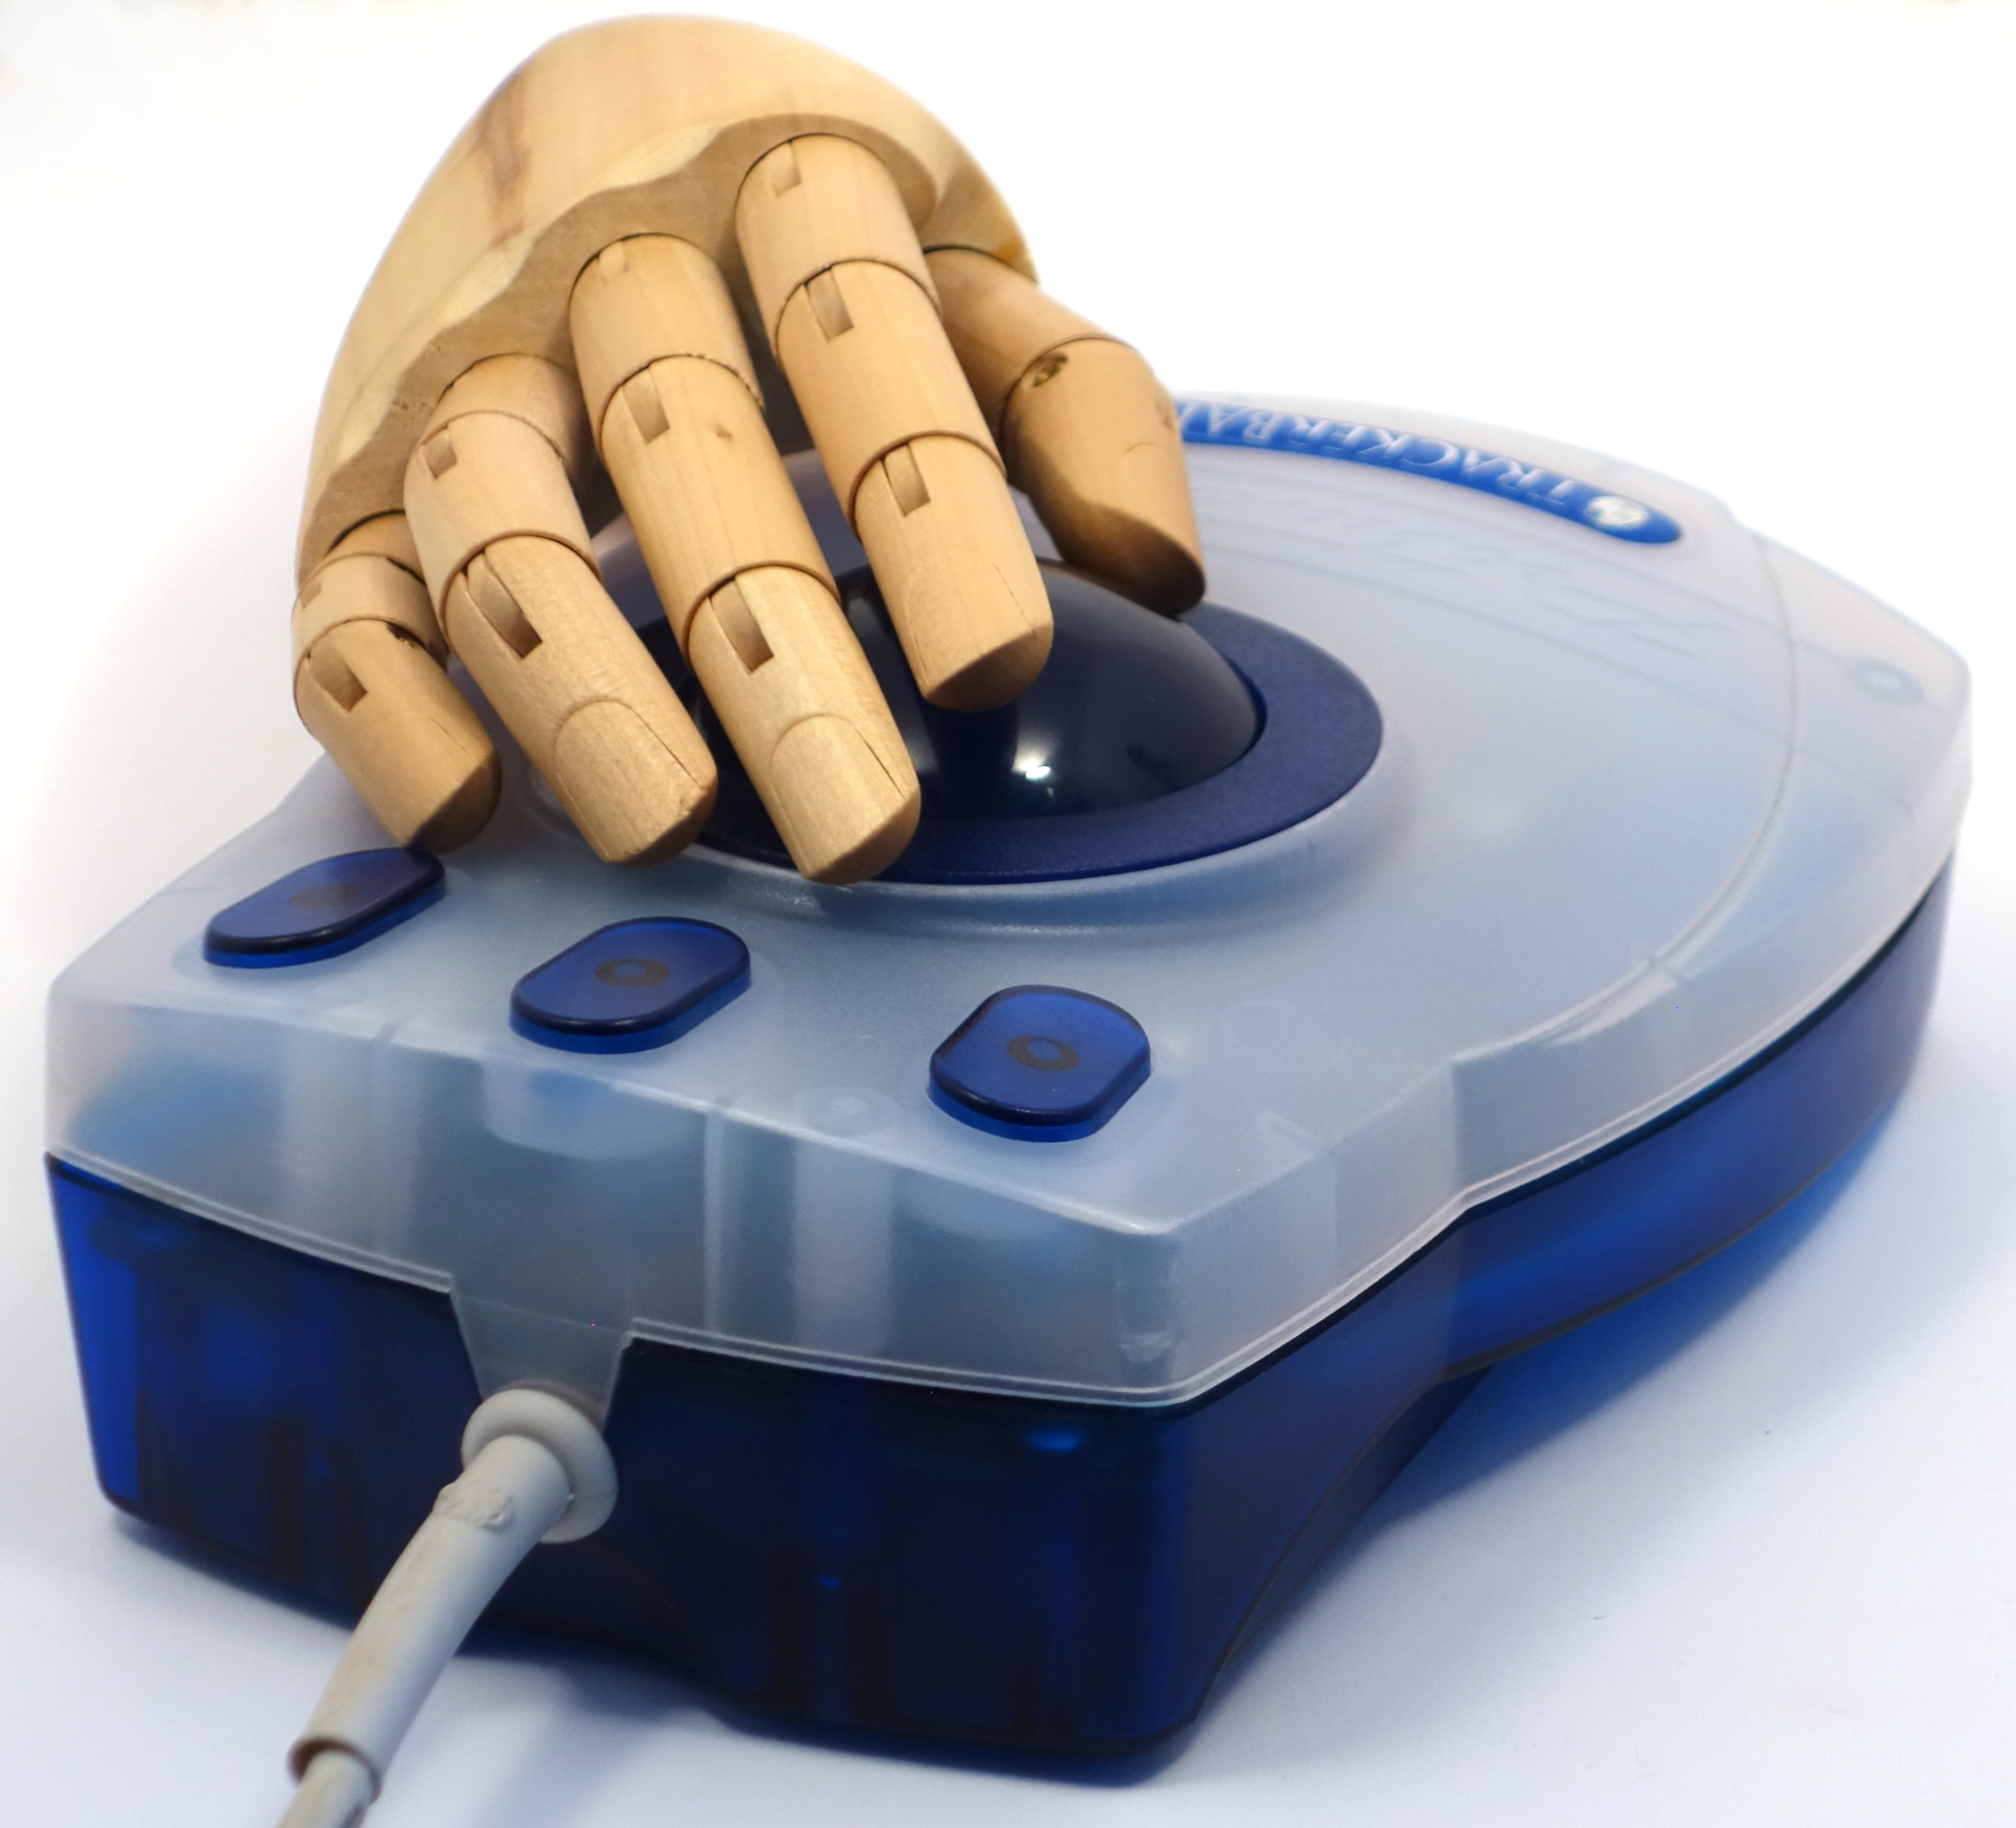
\includegraphics[scale=0.3]{1999_protrack_60i/raz_monstr_60.jpg}
    \caption{ProTrack 60i trackball with a human hand model}
    \label{fig:ProTrack60iHand}
\end{figure}

Figure \ref{fig:ProTrack60iTopBottom} shows top and bottom sides of the trackball.
The embossed “ProTrack 60i” text is present on the top of the case, as well as the “TRACKERBALL” emblem.

\begin{figure}[h]
    \centering
    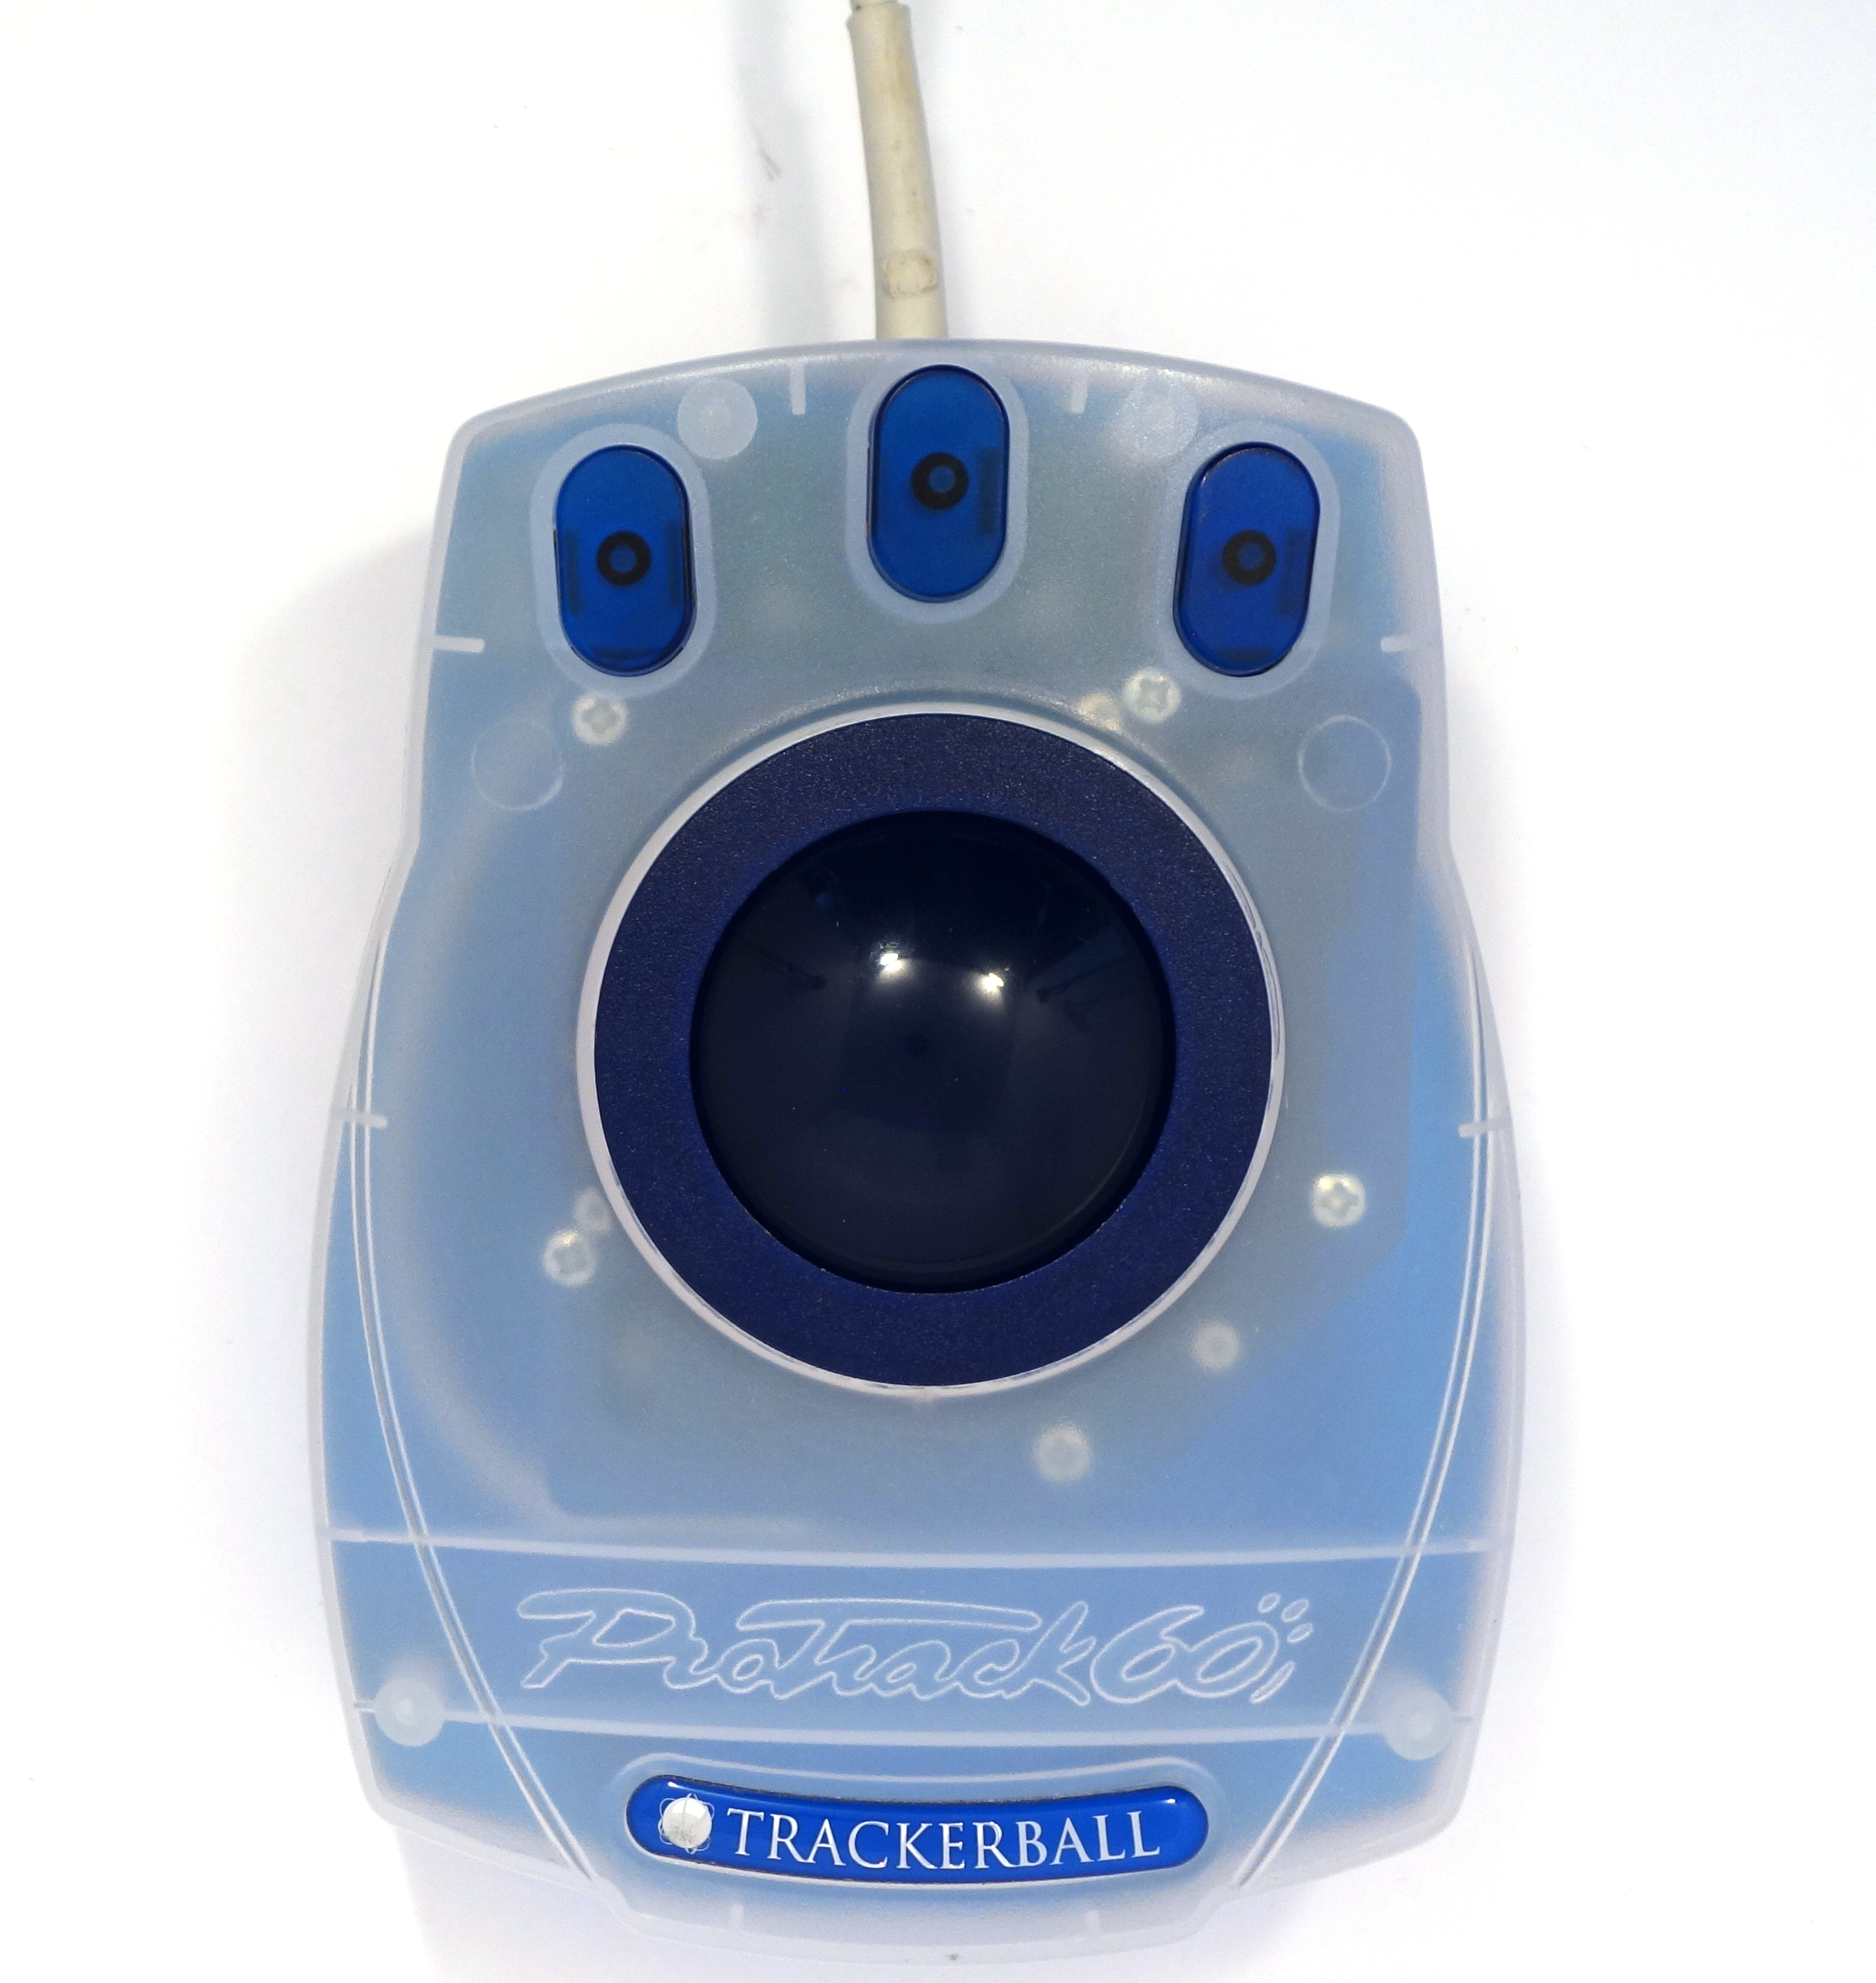
\includegraphics[scale=0.35]{1999_protrack_60i/monstr3_60.jpg}
    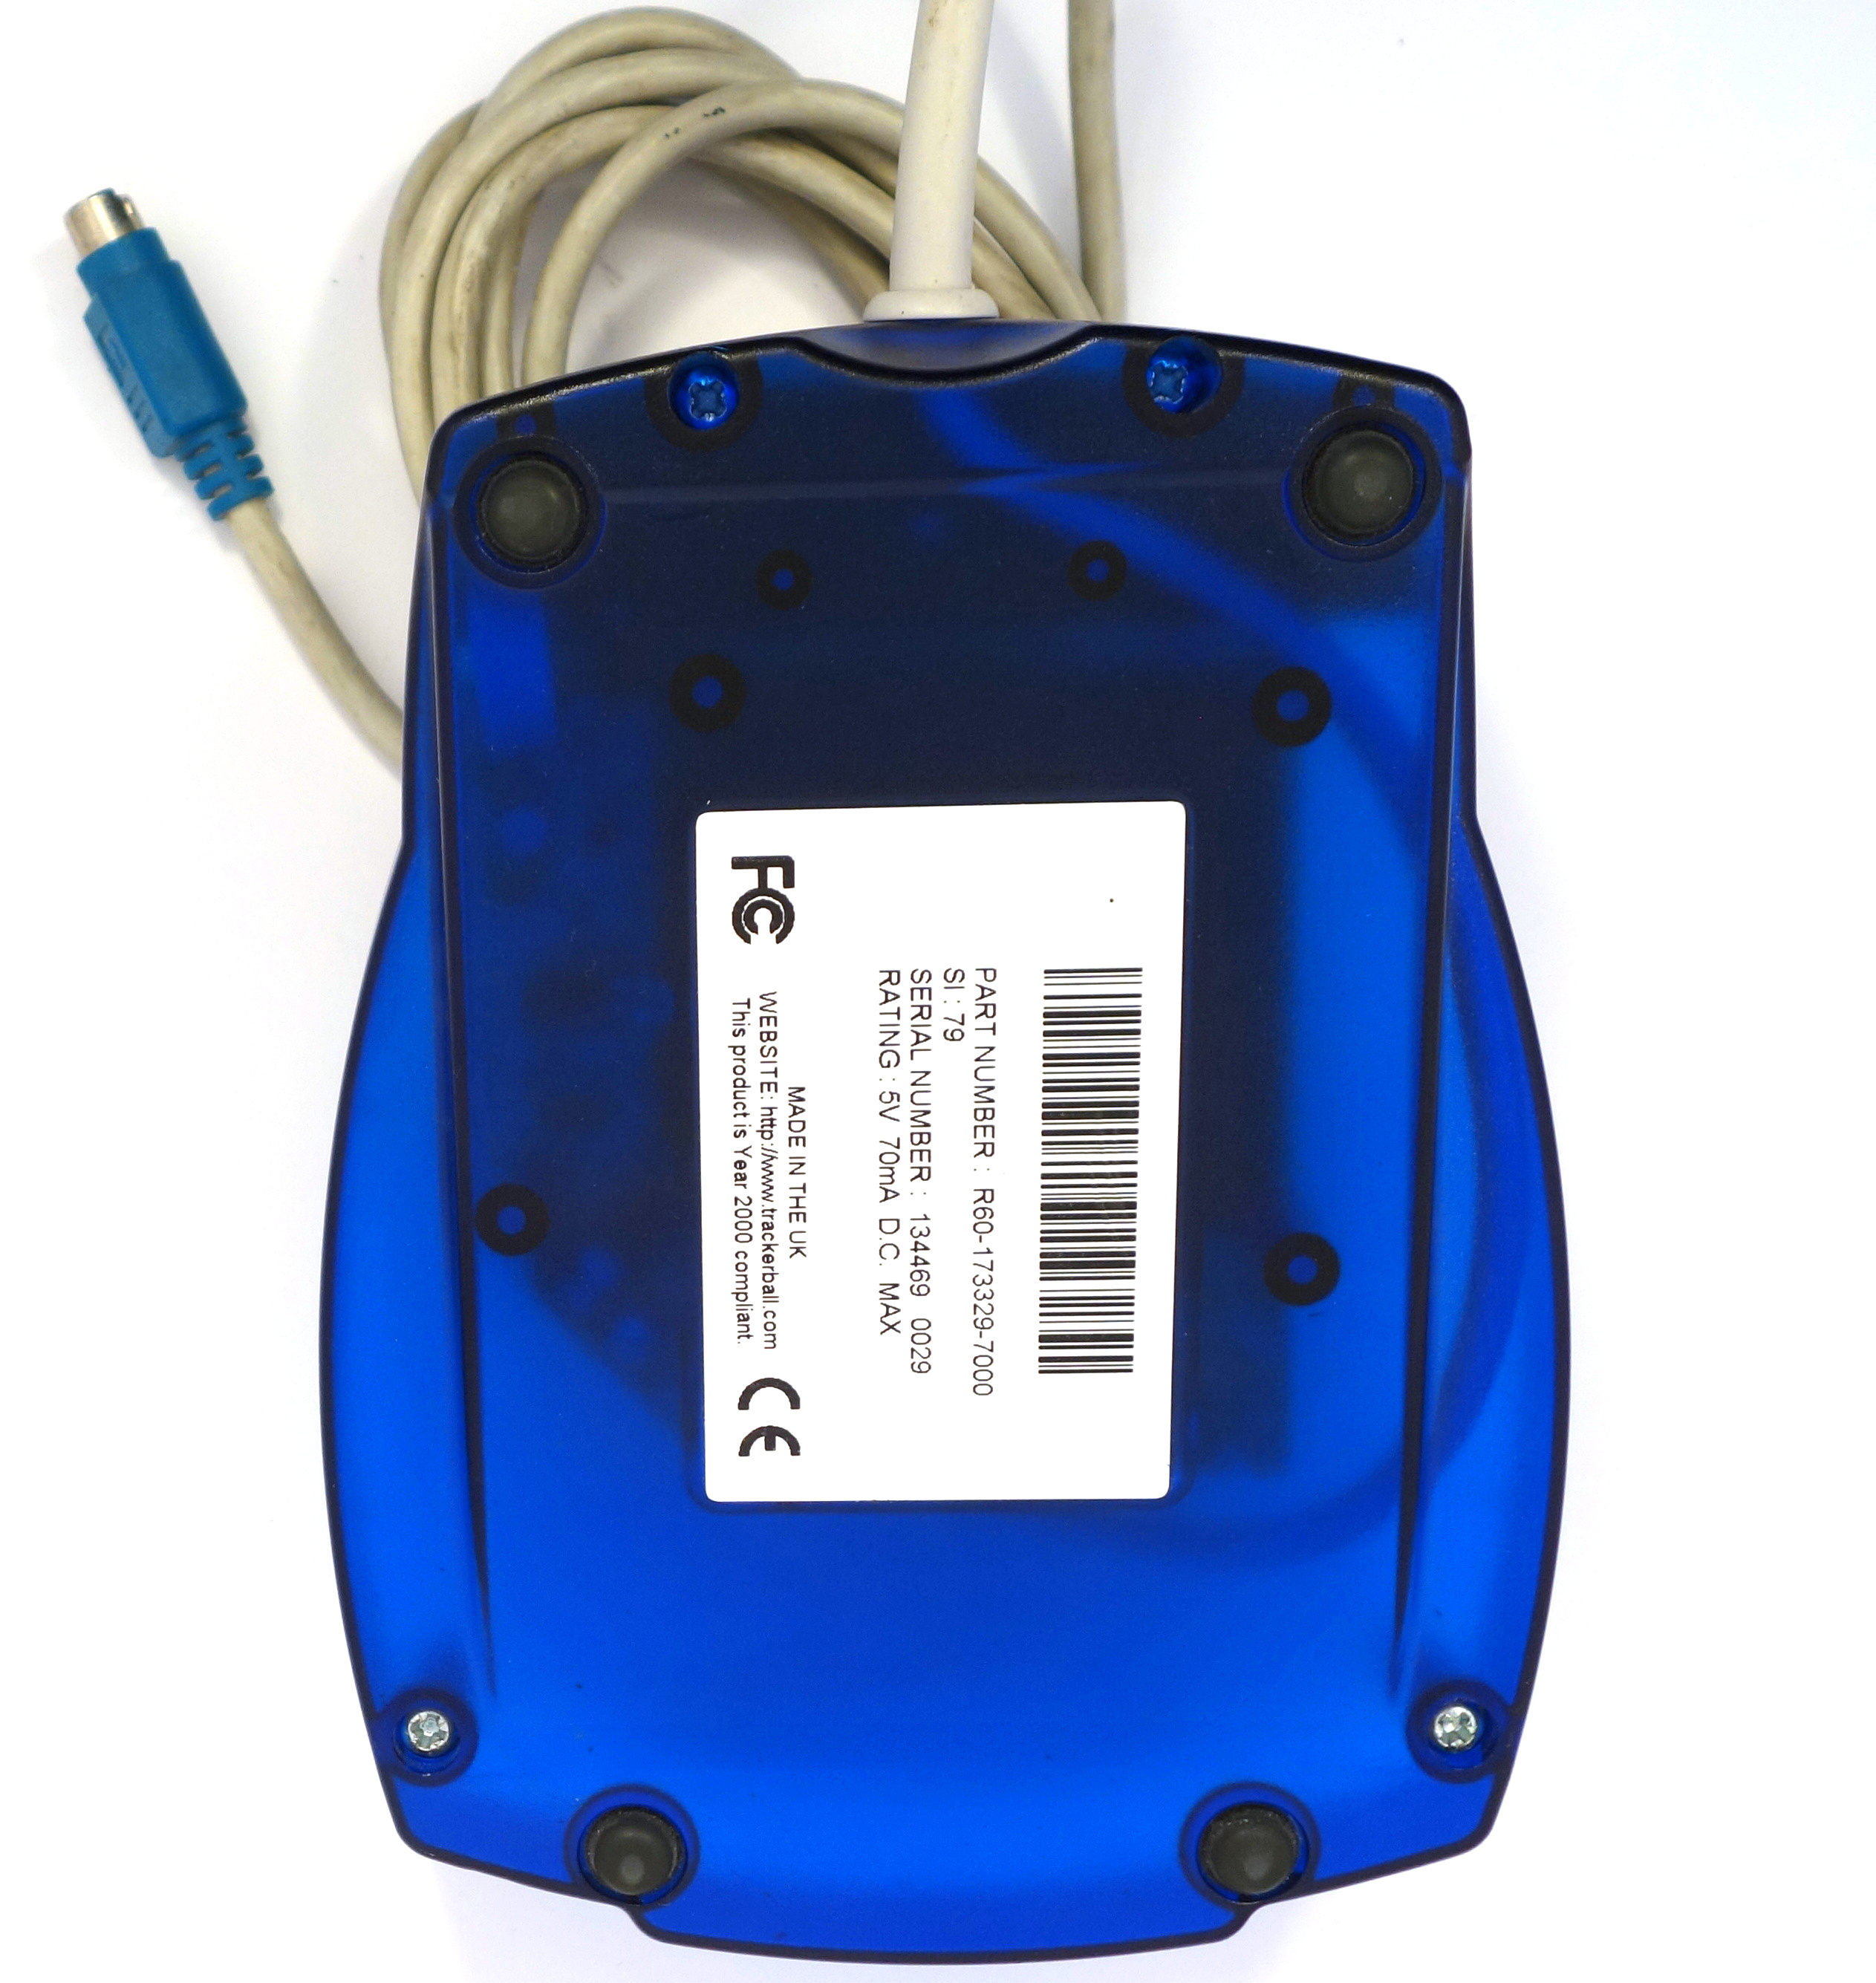
\includegraphics[scale=0.35]{1999_protrack_60i/monstr4_60.jpg}
    \caption{ProTrack 60i, top and bottom views}
     \label{fig:ProTrack60iTopBottom}
\end{figure}

Rubber feet are present on the underside of the case, fixing a secure position on the table surface, and there is also the ProTrack 60i marking. The country of manufacture of the device is United Kingdom.

\begin{figure}[h]
    \centering
    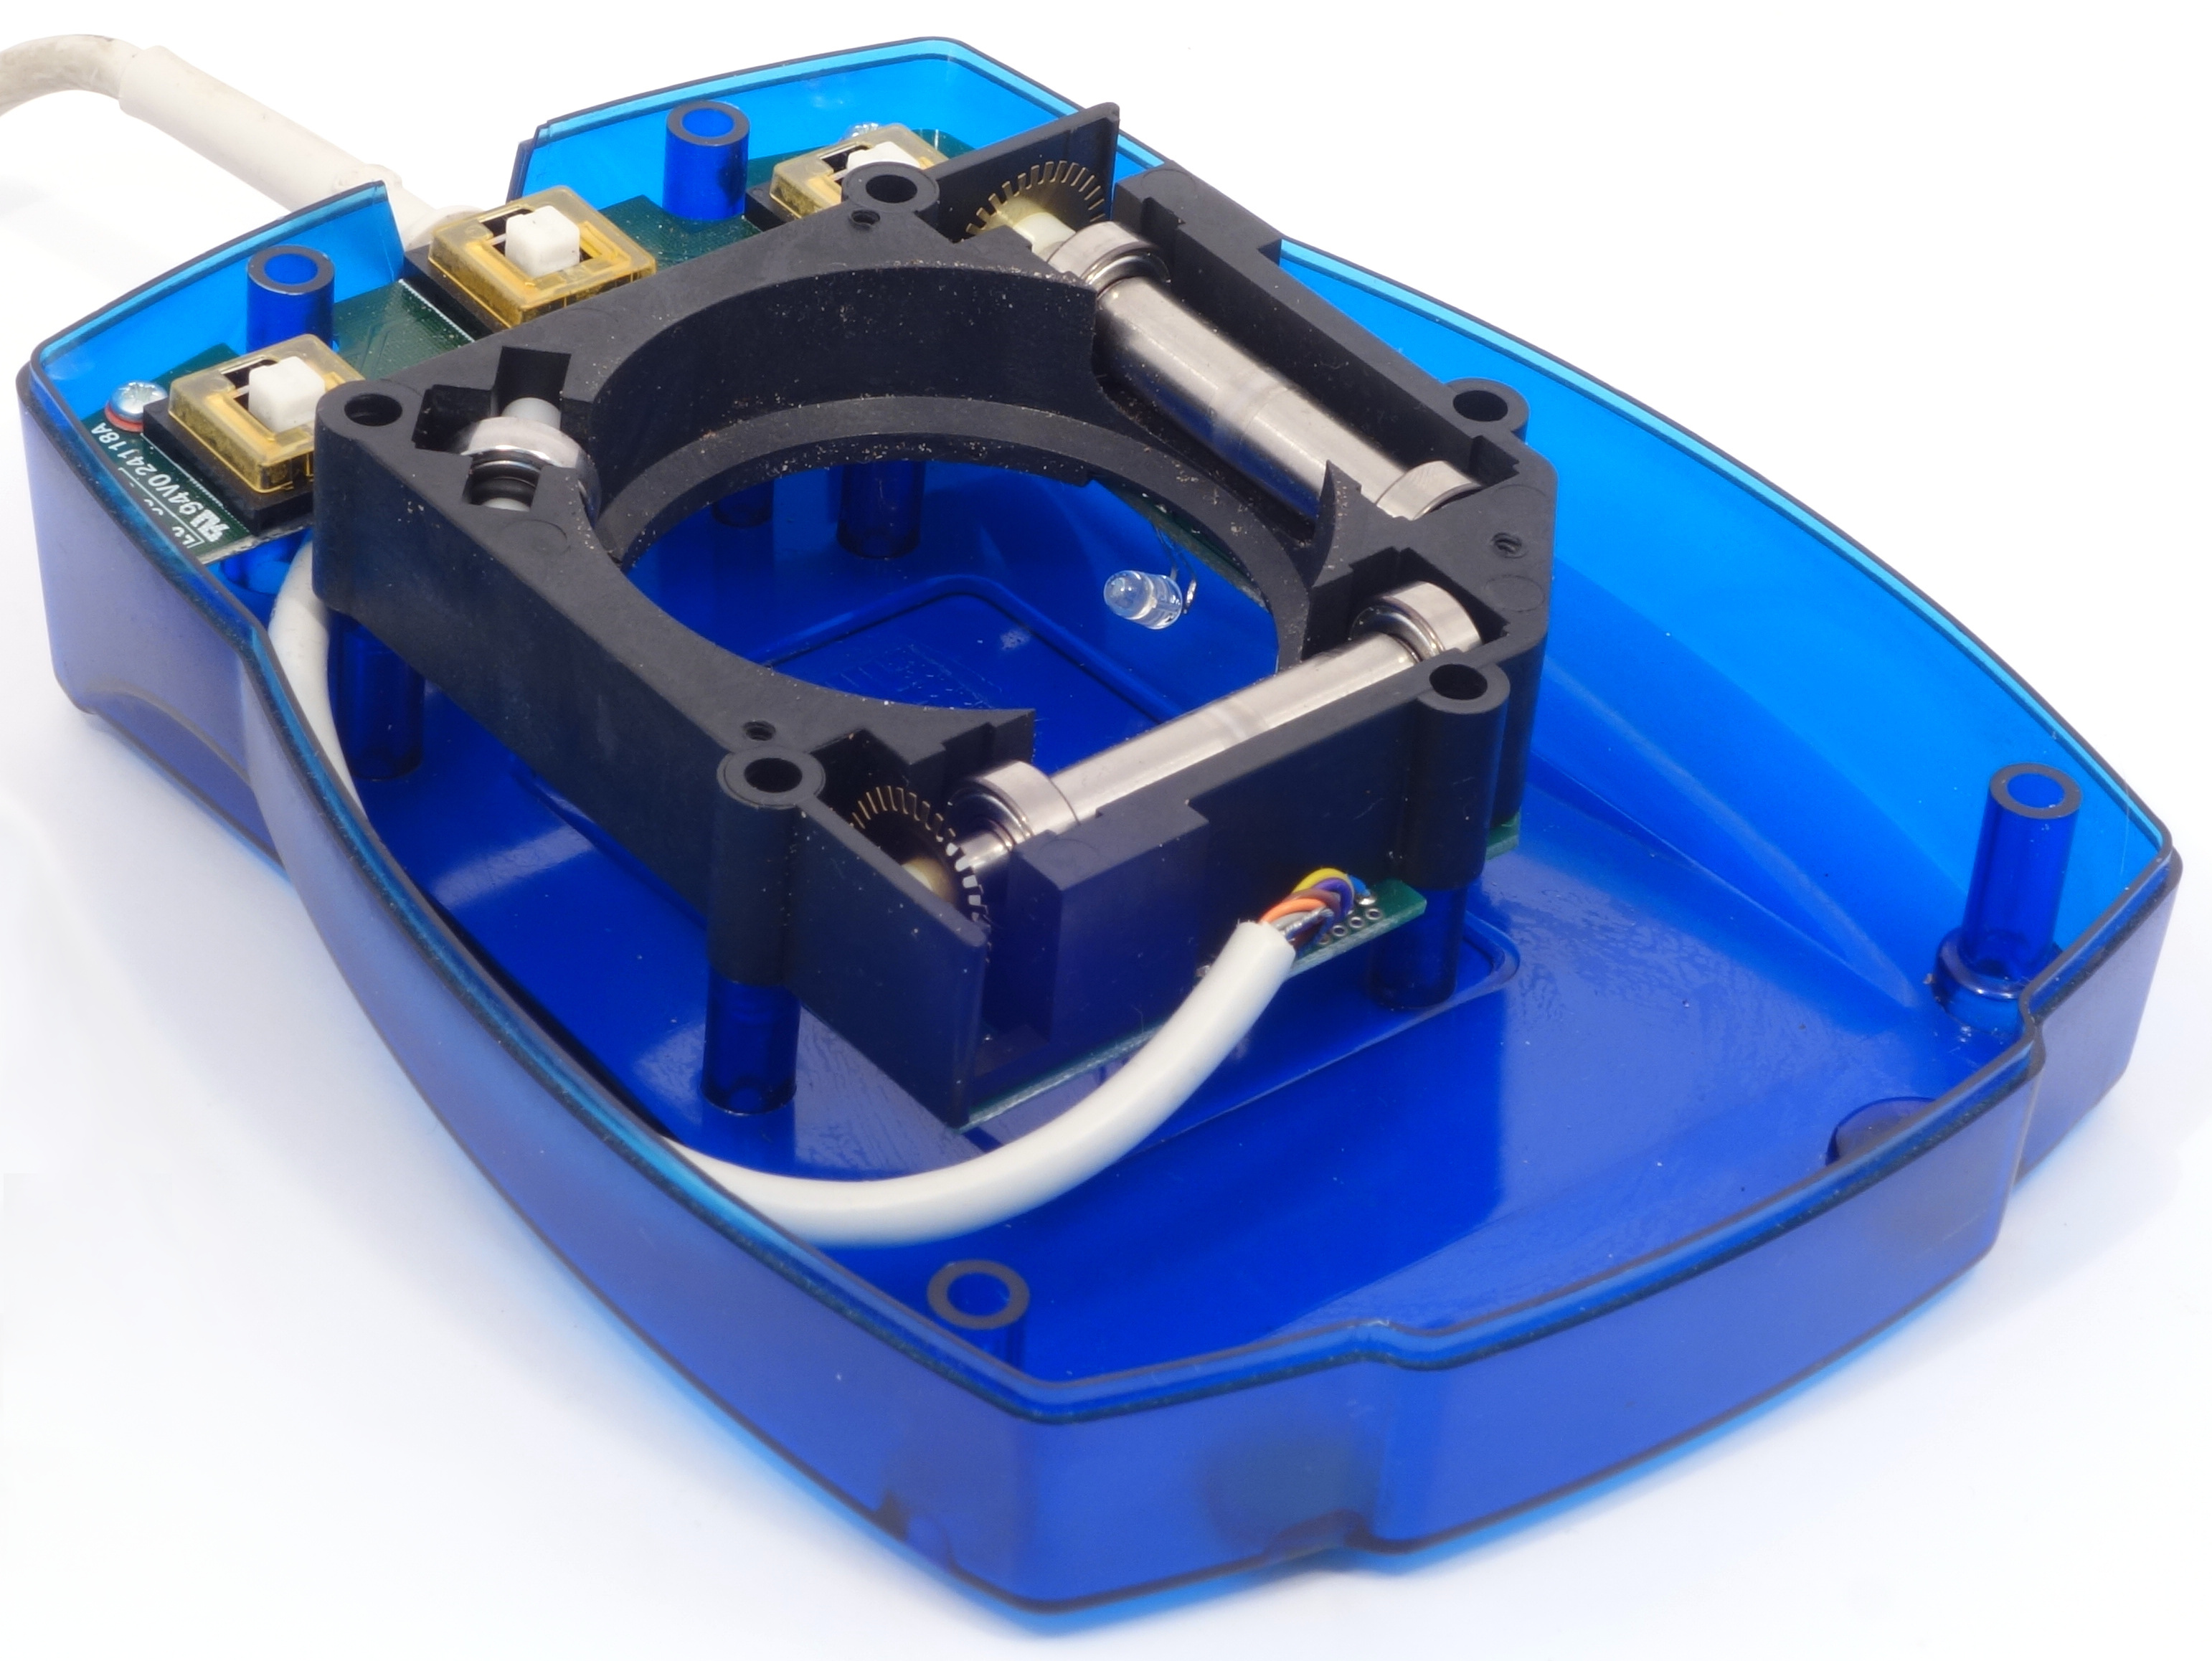
\includegraphics[scale=0.6]{1999_protrack_60i/razobr3_60.jpg}
    \caption{ProTrack 60i disassembled}
    \label{fig:ProTrack60iInside}
\end{figure}

Trackball internals are shown on figure \ref{fig:ProTrack60iInside}. As you can see, this trackball follows the traditional opto-mechanical scheme with an additional LED to highlight the ball. It should also be noted that the rollers are implemented using bearings and stainless steel shafts designed to ensure maximum reliability and durability of the device.
Apparently, it is impossible to get the ball out for cleaning without disassembling the case.

\begin{thebibliography}{9}
\bibitem{history} History of Cursor Controls, innovators in trackball manufacturing \url{https://www.cursorcontrols.com/about/history/}
\bibitem{trackerball} The Trackerball Company - Products \url{https://web.archive.org/web/19990128124617/http://www.trackerball.com/PRODUCT.HTM}
\bibitem{cursorcontrols} Cursor Controls Protrack 60 Industrial \url{https://web.archive.org/web/20010311155954/http://www.cursorcontrols.com/protrack60i.htm}
\bibitem{trackballfan} Trackball Fan! Cursor Controls ProTrack 60i (R60i) \url{http://www.hykw.com/tbfan/reviews/protrack.shtml}
\end{thebibliography}
\end{document}
